\section{第九章 \quad 传热过程分析与换热器基础}

%\subsection{传热过程分析}

基本传热方程为 $\Phi=kA(t_{f1}-t_{f2})=kA\Delta t$ 这里的 $\Phi$：传热量或热流量。$k$：传热系数。$A$：传热面积。$t_{f1}$、$t_{f2}$：两侧流体温度。$\Delta t$：两侧流体间温差。

\pt{通过平壁的传热过程计算}

传热系数为 $\frac{1}{\frac{1}{h_1}+\frac{\delta}{\lambda}+\frac{1}{h_2}}$

\pt{通过圆筒壁的传热过程分析}

\pt{热阻}：管内对流热阻 $R_{hi}=\frac{1}{\pi l h_id_i}$，管壁导热热阻 $R_\lambda =\frac{\ln(d_o/d_i)}{2\pi l\lambda}$，管外对流热阻 $R_{ho}=\frac{1}{h_o \pi l d}$

分别以管外面为换热基准面 $k_o=\frac{1}{\frac{1}{h_
i}\frac{d_o}{d_i}+\frac{d}{2\lambda}\ln\left(\frac{d_o}{d_i}\right)+\frac{1}{h}_o}$ 和管内面为基准面 $k_i=\frac{1}{\frac{1}{h_i}+\frac{d_i}{2\lambda}\ln\left(\frac{d_o}{d_i}\right)+\frac{1}{h}_o\frac{d_i}{d_o}}$

总热流为 $\Phi = \frac{\pi l(t_{fi}-t_{fo})}{\frac{1}{h_id_i}+\frac{1}{2\lambda_1}\ln\left(\frac{d_{o2}}{d_{o1}}\right)+\frac{1}{h_od_{o2}}}$

改变外径，当 $d_{o2}=\frac{2\lambda_2}{h_0}=d_{\mathrm{cr}}$ 或者 $\mathrm{Bi}=\frac{d_{o2}h_o}{\lambda_2}=2$ 时导热系数最大，$d_\mathrm{cr}$ 被称为临界热绝缘直径。

\pt{通过球壳的传热过程分析}

\pt{热阻}：球内对流 $R_{h_i}=\frac{1}{4\pi h_i r_i^2}$，球壳 $R_{\lambda}=(\frac{1}{4\pi\lambda}(\frac{1}{r_1}-\frac{1}{r_o}$，球外对流 $R_{h_o}=\frac{1}{4\pi h_o r_o^2}$

以球壳外面为基准面 $k_o = \frac{1}{\frac{r_o^2}{h_i r_i^2} + \frac{r_o^2}{\lambda} \left( \frac{1}{r_i} \frac{1}{r_o} \right) + \frac{1}{h_o}}$\\ 以球壳内面为基准面 $k_i = \frac{1}{\frac{1}{h_i} + \frac{r_i^2}{\lambda} \left( \frac{1}{r_i} \frac{1}{r_o} \right) + \frac{r_i^2}{h_o r_o^2}}$

\pt{传热过程的强化}

强化传热的实质：
    分析影响传热过程的因素，使设备单位体积换热量增加。
基本关系：
    $\Phi=kA\Delta t_m$
当 $\Phi$ 和 $\Delta t_m$ 一定时：
    若 $k$ 增大，则所需 $A$ 减小。
    可缩小设备体积，减少金属耗量。
    应用：载人航天、潜艇、空调等。
当 $\Phi$ 和 $A$ 一定时：
    若 $k$ 增大，则所需 $\Delta t_m$ 减小。
    可减小热应力、增加寿命、控制表面温度。
    应用：电子元器件冷却等。
强化传热原则：
    应从热阻最大的环节入手。
    在许多传热过程中，对流传热热阻相对较大。
    强化对流传热的核心是减薄边界层、增加流体扰动。
课件用管内湍流关联式说明强化方向：
    $\mathrm{Nu}_f=0.023\mathrm{Re}_f^{0.8}\mathrm{Pr}_f^n$
    $hd/\lambda=0.023(\rho ud/\eta)^{0.8}(\eta c_p/\lambda)^n$
若取常见形式 $n=0.4$，可得到：
    $h=0.023\lambda^{0.6}c_p^{0.4}(\rho u)^{0.8}/(\eta^{0.4}d^{0.2})$
由上式可看出强化措施：
    提高流速 $u$。
    减小特征管径 $d$。
    改变流体物性，如 $\lambda$、$c_p$、$\eta$、$\rho$。

\pt{削弱传热}

目的：
    减少热量或冷量损失，节约能源；
    保持物体内部温度恒定，减少波动；
    提高低温设备表面温度，防止结霜；
    防止温度不均匀，减小热应力；
    保证正常工作环境。
削弱传热的应用：
    热力设备、工程管路；
    建筑节能；
    低温液化气体储存和运输；
    航天器返回过程中的热防护。

\divider

%\subsection{换热器简介}

{\centering
    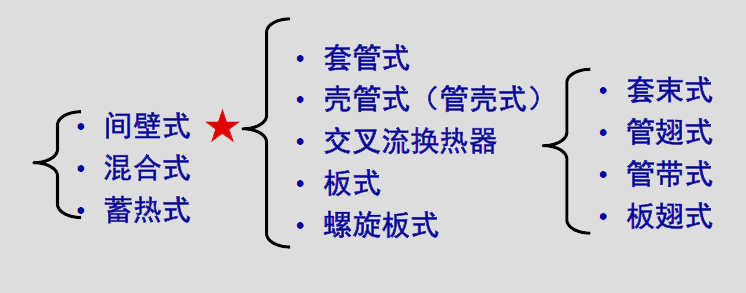
\includegraphics[width = \linewidth]{figures/9换热器的分类.png}
}

换热器的作用：
    使冷热流体之间发生热量交换。
    工程计算中通常使用传热系数 $k$、换热面积 $A$ 和平均温差 $\Delta t_m$ 来计算换热量。

套管式换热器：
    是最简单的一种间壁式换热器。
    流体可以顺流，也可以逆流。
    适用于传热量不大或流体流量不大的场合。

    管程与壳程：
    管内流动的通道称为管程。
    管外、壳体内流动的通道称为壳程。
管壳式换热器中的挡板：
    在同样流速下，流体横向掠过管子的换热效果比顺着管面纵向流过更强。
    因此外壳内常设置挡板，以改善壳程换热。
    挡板还可以支撑管子。
$1$-$2$ 型换热器：
    $1$ 表示 $1$ 个壳程。
    $2$ 表示 $2$ 个管程。
课件展示的管壳式结构：
    垂直折流板换热器。
    螺旋折流板换热器。
交叉流换热器：
    冷、热流体呈交叉方向流动。
    是间壁式换热器的重要形式之一。
    类型包括光管管束式、管翅式、管带式、板翅式。
交叉流换热器特点：
    常用于气体侧换热强化。
    翅片、板翅等结构可以显著增加换热面积。
板式换热器：
    由一组几何结构相同的平行薄平板叠加组成。
    冷、热流体间隔地在各通道中流动。
    特点是拆卸清洗方便。
    适用于含有易结垢物的流体。
课件展示的板式结构：
    平面板式换热器。
    螺旋板式换热器。

\pt{简单顺流及逆流换热器的对数平均温差}

换热器计算一般形式：
    $\Phi=kA\Delta t_m$
这里的 $\Delta t_m$ 不是简单取某一端温差，而是沿程温差的平均效果。
顺流换热器：
    冷、热流体从同一端进入。
    入口端温差较大，出口端温差较小。
    同侧端温差：
        $\Delta t'=t_1'-t_2'$
        $\Delta t''=t_1''-t_2''$
逆流换热器：
    冷、热流体从相反两端进入。
    沿程温差通常更均匀。
    同侧端温差：
        $\Delta t'=t_1'-t_2''$
        $\Delta t''=t_1''-t_2'$
符号说明：
    $t_1$ 表示热流体温度。
    $t_2$ 表示冷流体温度。
    $'$ 表示入口或一端状态。
    $''$ 表示出口或另一端状态。
【重点】对数平均温差：
    $\Delta t_m=(\Delta t_{\max}-\Delta t_{\min})/\ln(\Delta t_{\max}/\Delta t_{\min})$
    $\Delta t_{\max}$：同侧流体温差中的较大值。
    $\Delta t_{\min}$：同侧流体温差中的较小值。
对单侧流体与恒定壁温换热时，也可写成：
    $\Delta t_m=(t_f''-t_f')/\ln[(t_w-t_f')/(t_w-t_f'')]$
算术平均温差：
    $\Delta t_{m,\mathrm{算术}}=(\Delta t_{\max}+\Delta t_{\min})/2$
【重点】对数平均温差与算术平均温差的区别：
    算术平均温差相当于假定冷热流体温度沿程呈直线变化。
    在相同进出口温度下，算术平均温差总是大于或等于对数平均温差。
    对数平均温差更符合实际换热过程。
计算时的基本步骤：
    判断流动方式是顺流还是逆流。
    写出两端同侧温差。
    找出 $\Delta t_{\max}$ 与 $\Delta t_{\min}$。
    代入对数平均温差公式。
    再由 $\Phi=kA\Delta t_m$ 求换热量或面积。
